\documentclass{article}

\usepackage{amsmath, amsthm, amssymb, amsfonts}
\usepackage{thmtools}
\usepackage{graphicx}
\usepackage{setspace}
\usepackage{geometry}
\usepackage{float}
\usepackage{hyperref}
\usepackage[utf8]{inputenc}
\usepackage[english]{babel}
\usepackage{framed}
\usepackage[dvipsnames]{xcolor}
\usepackage{tcolorbox}

\colorlet{LightGray}{White!90!Periwinkle}
\colorlet{LightOrange}{Orange!15}
\colorlet{LightGreen}{Green!15}
\colorlet{LightBlue}{Blue!15}
\colorlet{LightRed}{Red!15}



\newcommand{\HRule}[1]{\rule{\linewidth}{#1}}
\newcommand{\N}{\mathbb{N}}
\newcommand{\R}{\mathbb{R}}

\declaretheoremstyle[name=Theorem,]{thmsty}
\declaretheorem[style=thmsty,numberwithin=section]{theorem}
\tcolorboxenvironment{theorem}{colback=LightGray}

\declaretheoremstyle[name=Proposition,]{prosty}
\declaretheorem[style=prosty,numberlike=theorem]{proposition}
\tcolorboxenvironment{proposition}{colback=LightOrange}

\declaretheoremstyle[name=Definition,]{definsty}
\declaretheorem[style=definsty,numberlike=theorem]{definition}
\tcolorboxenvironment{definition}{colback=LightGreen}

\declaretheoremstyle[name=example,]{examsty}
\declaretheorem[style=examsty,numberlike=theorem]{example}
\tcolorboxenvironment{example}{colback=LightRed}

\declaretheoremstyle[name=remark,]{Remarksty}
\declaretheorem[style=Remarksty,numberlike=theorem]{remark}
\tcolorboxenvironment{remark}{colback=LightBlue}

\setstretch{1.2}
\geometry{
    textheight=9in,
    textwidth=5.5in,
    top=1in,
    headheight=12pt,
    headsep=25pt,
    footskip=30pt
}

% ------------------------------------------------------------------------------

\begin{document}

% ------------------------------------------------------------------------------
% Cover Page and ToC
% ------------------------------------------------------------------------------

\title{ \normalsize \textsc{}
		\\ [2.0cm]
		\HRule{1.5pt} \\
		\LARGE \textbf{\uppercase{Analysis}
		\HRule{2.0pt} \\ [0.6cm] \LARGE{Study Note} \vspace*{10\baselineskip}}
		}
\date{}
\author{\textbf{Author} \\ 
		Sam Ren \\
		Grinnell College \\
		\today }

\maketitle
\newpage

\tableofcontents
\newpage

% ------------------------------------------------------------------------------

\section{Pre-knowledge}
\subsection{Fundamentals of Logic}
Symbolic logic is about statements which one can meaningfully claim to be true or false. That is, each statement has the truth value 'True'(T) or 'false' (F). (By Analysis I from Herbert)
\begin{theorem}
	A statement is either True or False. There are no other possibilities, and no statement can be both true and false.
\end{theorem}

\subsection{Sets}
\begin{definition}
	Power sets($P(X)$) are the set of all subset of $X$.
\end{definition}

There are serval properties
\begin{itemize}
	\item $\emptyset\in  P(X)$
	\item $X\in P(X)$
	\item $x\in X\Leftrightarrow {x}\in P(X)$
	\item $Y\subseteq X \Leftrightarrow Y\in P(X)$
\end{itemize}


\begin{definition}
	(Cartesian) product$X\times Y$ of two sets $X,Y$ are set of order pairs$(x,y)$ where $x\in X,y\in Y$ 
\end{definition}

\begin{definition}
	Families of Sets$A_\alpha$ is a set which have index $\alpha$ where $\alpha\in A$ and $A$ is nonempty
\end{definition}

\subsection{Functions}
\begin{definition}
	A function, map $f$ from set $X$ to $Y$ is a kind of rule which for each element in set $X$ specifies exactly one element in $Y$, we denote as:
	\begin{equation*}
		f:X\to Y
	\end{equation*}
	Where the element in $Y$ is $f(x)$ we call it the value of $f$ at $x$, and we call $X$ as the domian of the function, $Y$ as the codomain of the $f$
\end{definition}

\begin{definition}
	Image of $f$ is a subset of $Y$ for $f: X\to Y$ where defined as:
	\begin{equation*}
		\text{im}(f):=\{y\in Y, \exists x\in X:y=f(x) \}
	\end{equation*}
	
\end{definition}

I am now going to give some basic function we might use later:
\begin{itemize}
	\item Projection: If $X_1,....,X_i$ are not empty then the projection function is \begin{equation*}
		pr_k: \prod_{j=1}^n X_j \to X_k ,\ x=(x_1,...,x_n)\to x_k,\ k=1,2,3,...
	\end{equation*}
	\item characteristic function: Let $X\neq \emptyset$, and $A\subseteq X$. Then the characteristic function of $A$ is:\begin{equation*}
		\chi_A: X\to \{0,1 \}, x\to 
	\end{equation*}
\end{itemize}


\subsection{Injections, Surjections and Bijections}





\subsection{Limits}
%-------------------------------------------------------------------------
\subsection{Limits of Sequence}
\begin{definition}{Limit of Sequence}
The limit of a sequence $(a_n)$ is defined as follows: $\forall \varepsilon > 0, \exists N$ such that for all $n > N$,
\begin{equation*}
|a_n - L| < \varepsilon
\end{equation*}
The limit of the sequence is $L$, denoted as $\lim_{n\to \infty}a_n = L$.
\end{definition}
Here is an illustration of this definiton:
\begin{figure}[h]
	\centering
	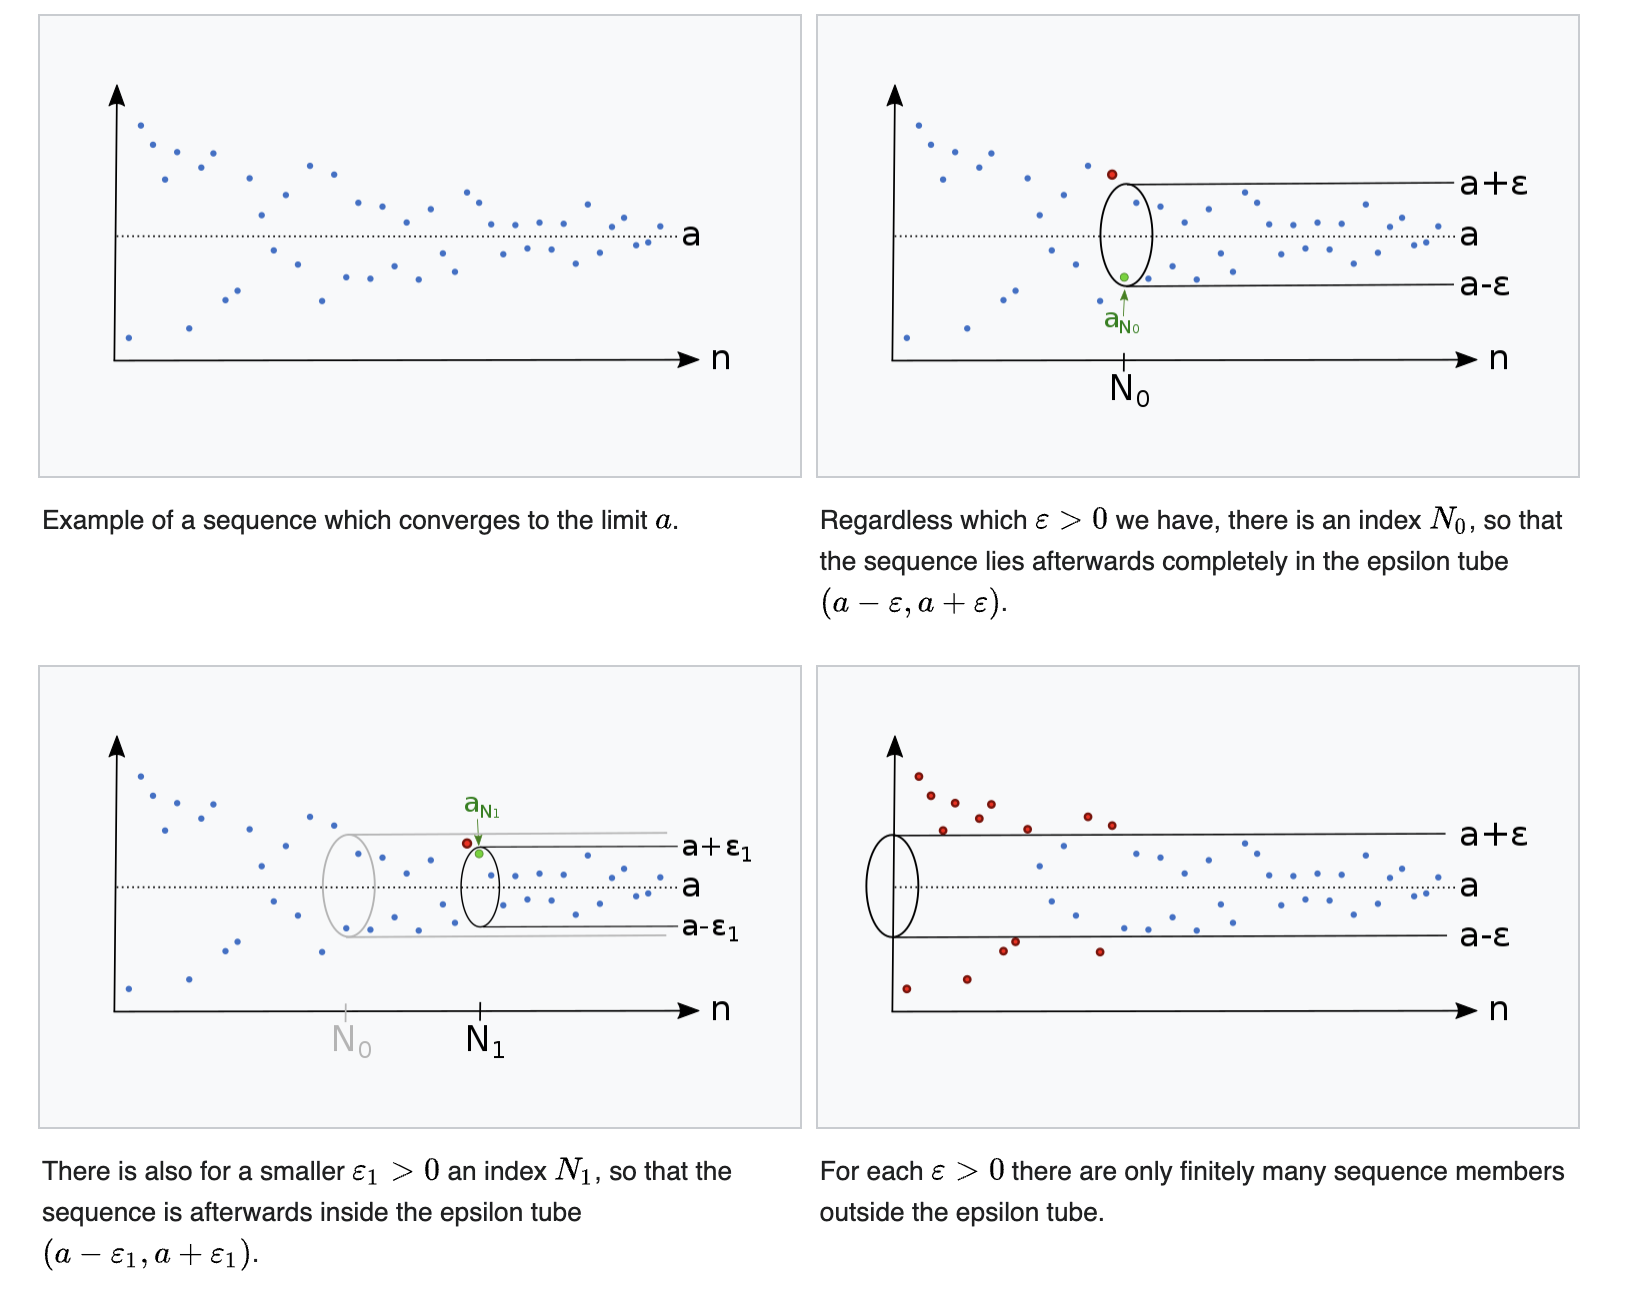
\includegraphics[scale=0.35]{img/seqlimit.png}
\end{figure}


If a sequence $(a_n)$ has a limit, then it is a convergent sequence; otherwise, it is a divergent sequence.

\begin{theorem}
The limit of a sequence possesses several important properties, including:
\begin{enumerate}
\item The limit of a sequence is unique.
\item If $a_n \leq b_n$ for all $n$ greater than some $N$, and both sequences have finite limits, then $\lim_{n\to \infty}a_n \leq \lim_{n\to \infty}b_n$.
\end{enumerate}
\end{theorem}

For further exploration: If $a_n > 0$ for all $n > N$, and the limit of $a_n$ as $n$ approaches infinity exists and is finite, then this limit is greater than 0.



\subsection{Limits of function}









\section{Numbers}
\subsection{The Natural Numbers}
\subsection{The Peano Axioms}
The natural number consist with set $\N$, where a distinguished element 0 $\in \N$, and a function $\nu : \N \to \N^{\times}:=\N \backslash \{0\}$ with following properties:
\begin{enumerate}
	\item $\nu$ is injective
	\item If a subset $N$ contains 0 and $\nu(n)\in N$ for all $n\in N$ then $N=\N$ 
\end{enumerate}

And we denote 






\section{Real analysis}
\subsection{Construction of the real numbers}
\subsubsection{Completeness of Real number}

Can you prove the "irrationality property" for the following set of numbers?

We know $\sqrt{2}$ is irrational. We need to prove that the set 
$L = \{ x \leq 0 \} \cup \{ x > 0 : x^2 < 2 \}$, 
together with the set $R = \{ r > 0 : r^2 > 2 \}$, 
are disjoint subsets of the rational numbers $\mathbb{Q}$, 
and that for every $r \in R$ there exists a "gap", 
i.e., there is no number in $L$ such that it is one less than any number in $R$. 
Formally, this is described as: for every $x \in (-\infty, \sqrt{2})$ 
and $(\sqrt{2}, +\infty)$, there is no rational number equal to $\sqrt{2}$.

Here are the conditions for a set $A$ and $B$ to prove the irrationality property, 
with $A$ and $B$ being nonempty subsets of $\mathbb{Q}$, disjoint and open:

\begin{enumerate}
  \item If $a \in A$, then there exists an $a' \in A$ such that $a' > a$.
  \item If $b \in B$, then there exists a $b' \in B$ such that $b' < b$.
  \item If $a \in A$ and $b \in B$, then $a \leq b$.
  \item There are no largest or smallest elements in $A$ or $B$.
\end{enumerate}

Since $L = A \cap \mathbb{Q}$ and $R = B \cap \mathbb{Q}$ are nonempty and consist of all rational numbers less than or equal to $\sqrt{2}$ and greater than $\sqrt{2}$ respectively, then according to the property above, we can define the set $A = (-\infty, \sqrt{2}) \cap \mathbb{Q}$, $B = (\sqrt{2}, +\infty) \cap \mathbb{Q}$.

Therefore, for $a \in A$ and $b \in B$, we have $a \leq x < \sqrt{2} < b$. Finally, since $A = (-\infty, x)$ and $B = [x, +\infty)$.







\clearpage
\subsection{Order properties of the real numbers}
\clearpage

\subsection{Sequences}
\subsection{Supremum \& Infimum}

\begin{definition}
	For a subset $M\subseteq \R$, $b\in \R$ is called Upper bound iff:
	\begin{equation*}
		\forall x\in M: x\leq b
	\end{equation*}
	If it is a lower bound, then $x\geq b$
\end{definition}

In simpler terms, an upper bound is a value that is greater than or equal to every element in the set.

\begin{definition}
	For a subset $M\subseteq \R$, $s\in \R$ is called supremum iff:
	\begin{itemize}
		\item $\forall x\in M: x\leq s$
		\item $\forall \varepsilon >0, \exists \bar{x}\in M : s-\varepsilon< \bar{x}$
	\end{itemize}
	Then we write $\sup M := s$
\end{definition}



\begin{definition}
		For a subset $M\subseteq \R$, $l\in \R$ is called infimum iff:
	\begin{itemize}
		\item $\forall x\in M: x\geq l$
		\item $\forall \varepsilon >0, \exists \bar{x}\in M : l+\varepsilon> \bar{x}$
	\end{itemize}
	Then we write $\inf M := l$
\end{definition}

\begin{remark}
	If $M$ is not bounded, then we write $\sup M:= \infty, \inf M:=-\infty $.
	
	If $M$ is an empty set, then we write $\sup M:= -\infty, \inf M:=\infty$
\end{remark}

\subsection{Cauchy sequence}\label{Cauchy sequence}

\begin{definition}
	A sequence $(a_n)_{n\in \mathbb{N}}$ is called cauchy sequence iff:
	\begin{equation*}
		\forall \varepsilon >0, \exists N\in \mathbb{N}, \forall n,m\geq N: |a_n-a_m|<\varepsilon
	\end{equation*}
\end{definition}

In simpler terms, this means that as you move further along in the sequence, the difference between its terms becomes smaller and smaller, eventually becoming as small as you like. 
\begin{remark}
	In real numbers, every convergent sequence is a Cauchy sequence, and every Cauchy sequence is convergent. This equivalence is a cornerstone of real analysis.
	\begin{equation*}
		\text{Cauchy sequence} \Leftrightarrow \text{Convergent sequence}
	\end{equation*}
	Which is known as completeness axiom.
\end{remark}

\begin{theorem}
	Dedekind completeness: 
	\begin{itemize}
		\item If $M\subseteq \R$ is upper bounded, then $\sup M\in \R$ exists
		\item If $M\subseteq \R$ is lower bounded, then $\inf M\in \R$ exists
	\end{itemize}
\end{theorem}

\begin{proof}
	Not yet understand()
\end{proof}

\begin{theorem}
	If a sequence is monotonically decreasing and bounded below, then it is a convergent sequence.
\end{theorem}

\subsection{Bolzano-Weierstrass Theorem}
\begin{theorem}
	If $(a_n)_{n\in \mathbb{N}}$ is bounded, then it has a accumlation value. In another word, every bounded sequence in real number has a convergent subsequence.
\end{theorem}

\begin{proof}
	Lets define a new sequence which has lower bound $c_0$ and upper bound $d_0$. Then we can esaily divide it into bisection with two same interval. 
	
\textbf{Bisection step:}	At least one of these subintervals must contain infinitely many terms of the sequence \((a_n)\). Label this subinterval as \([c_1, d_1]\). Repeat this process for \([c_1, d_1]\), dividing it into two and selecting the subinterval, say \([c_2, d_2]\), that contains infinitely many terms of \((a_n)\). Continue this process indefinitely. In each step, select a subinterval \([c_k, d_k]\) that contains infinitely many terms of the sequence. 

\textbf{Limit step} After we get the $[c_k,d_k]$, we can see that, $[c_k, d_k]\subset [c_{k-1}, d_{k-1}]\subset [c_{k-2}, d_{k-2}]\subset ...\subset [c_0, d_0]$. Hence, $d_1-c_1=\frac{1}{2}(d_0-c_0),d_n-c_n=\frac{1}{2^n}(d_{n-1}-c_{n-1})$. When $n\to \infty$, the difference apporach to 0. 

\textbf{Construction step:} It is obvious that $(c_n)_{n\in \mathbb{N}}$ is monotonically increase and $(d_n)_{n\in \mathbb{N}}$ is monotonically decrease. That is, they are convergent. (After prove they are convergent we can apply limit on these sequences) Notice:
\begin{equation*}
	\lim_{n\to \infty}(d_n-c_n)=0=\lim_{n\to \infty}(d_n)-\lim_{n\to \infty}(c_n)
\end{equation*}

\textbf{Final step:} Then let's define $(a_{n_k})_{k\in \mathbb{N}}$ as a new sequence where $a_{n_k}\in [c_k,d_k]$. That is:
\begin{equation*}
	c_k\leq a_k\leq d_k
\end{equation*}
By sandwich theorem we know that $(a_{n_k})_{k\in \mathbb{N}}$ is convergent.

\end{proof}


\subsection{Limit superior and inferior}
\begin{equation*}
	\begin{aligned}
		&\lim_{n\to \infty}a_n=\infty \Leftrightarrow \text{Divergent to }\infty \Leftrightarrow  \forall C>0, \exists N\in \mathbb{N}, \forall n\in N: a_n>C\\
		&\lim_{n\to \infty}a_n=-\infty \Leftrightarrow \text{Divergent to }-\infty \Leftrightarrow  \forall C<0, \exists N\in \mathbb{N}, \forall n\in N: a_n<C
	\end{aligned}
\end{equation*}

We call this type of accumulation as improper accumulation. When it does not bounded lower, then it has improper value of $-\infty$, when it does not bounded above, then it has improper value of $\infty$.

\begin{definition}
	For sequence $(a_n)_{n\in \mathbb{N}} $, An element $a\in \R \bigcup \{-\infty,\infty \}$ is called:
	\begin{itemize}
		\item Limit superior of $(a_n)_{n\in \mathbb{N}} $ if $a$ is the largest (improper) accumulation value of $(a_n)_{n\in \mathbb{N}} $. We write: $a=\limsup_{n\to \infty}a_n$
		\item Limit inferior of $(a_n)_{n\in \mathbb{N}} $ if $a$ is the smallest (improper) accumulation value of $(a_n)_{n\in \mathbb{N}} $. We write: $a=\liminf_{n\to \infty}a_n$
	\end{itemize}
	At the same time we can write:
	\begin{equation*}
		\limsup_{n\to \infty}a_n=\lim_{n\to \infty}\sup\{a_k | k\geq n \}
	\end{equation*}
		\begin{equation*}
		\liminf_{n\to \infty}a_n=\lim_{n\to \infty}\inf\{a_k | k\geq n \}
	\end{equation*}
\end{definition}

There are serval researons for define the limit superior and limit inferior
\begin{itemize}
	\item For sequences that do not converge, the limit superior and inferior provide a way to describe their behavior. They are particularly useful in handling oscillating sequences or sequences with multiple limit points. 
	\item Unlike the usual limit, the limit superior and limit inferior always exist for any bounded sequence and for many unbounded sequences.
	\item If a sequence $a_n$ does converge, then its limit superior and limit inferior are both equal to this limit. This property is often used in proofs to show convergence.
	\item These concepts are also used in the convergence tests for series, particularly in understanding the behavior of the terms of a series.
\end{itemize}

\begin{example}
	\begin{equation*}
		a_n=(-1)^n\cdot n= -1,2,-3,...
	\end{equation*}
	It is obvious that this sequence is not convergent however we can find a subsequence where we can esaily get the limit superior and inferior:
	\begin{equation*}
		\limsup_{n\to \infty}a_n=\infty
	\end{equation*}
	\begin{equation*}
		\liminf_{n\to \infty}a_n=-\infty
	\end{equation*}
\end{example}

\begin{theorem}
	Sequence $a_n$ is conergent if:
	\begin{equation*}
		\limsup_{n\to \infty}a_n=\liminf_{n\to \infty}a_n \notin \{\infty,-\infty \}
	\end{equation*}
	At the same time, if $a_n$ is divergent to $\infty$ then:
	\begin{equation*}
		\limsup_{n\to \infty}a_n=\liminf_{n\to \infty}a_n=\infty
	\end{equation*}
\end{theorem}

Some properties which are only exists when the value is defined(Not infinty times zero etc.):
\begin{enumerate}
	\item $\limsup_{n\to \infty}(a_n+b_n)\leq \limsup_{n\to \infty}a_n+\limsup_{n\to \infty}b_n$
	\item $\limsup_{n\to \infty}(a_n\cdot b_n)\leq \limsup_{n\to \infty}a_n\cdot \limsup_{n\to \infty}b_n$
\end{enumerate}

For limit inferior, we just change the direction of inequality.
\clearpage
\subsection{Series}
\begin{definition}
Series are sequence($S_n$) which is the summation of a sequence $a_n$ from inital value to infinity, where we denote it as:
	\begin{equation*}
		S_n=\sum_{i=1}^n a_i,n\in \mathbb{N}
	\end{equation*}
	If $S_n$ is convergent then we write: 
	\begin{equation*}
		\sum_{i=1}^\infty a_i:=\lim_{n\to \infty} S_n=\lim_{n\to \infty}\sum_{i=1}^\infty a_i
	\end{equation*}
\end{definition}


\begin{example}
Harmonic series are special series which write as:
\begin{equation*}
	\sum_{k=1}^\infty \frac{1}{k}
\end{equation*}	
This serie seems to be convergent however it is not.
\end{example}

\begin{proof}
	Let $S_n=\sum_{k=1}^n \frac{1}{k}$ where increase monotonically and we are going to prove that this sequence is not bounded above. 
\end{proof}

Here are some properties if series $\sum a_k, \sum b_k$ are convergent
\begin{enumerate}
	\item $\sum(a_k+b_k)=\sum a_k  +\sum b_k$ convergent
	\item $\sum (\lambda a_k)=\lambda \sum a_k$
\end{enumerate}


\subsubsection{Criterion of Series}
\begin{theorem}
	Cauchy criterion claims that a series in $\R$ is convergent iff it is cauchy sequence and follows that:
	\begin{equation*}
	\sum^\infty a_k \text{Convergent} \leftrightarrow \forall \varepsilon >0, \exists N\in \N, \forall n\geq m\geq N
	\end{equation*}
	we have:
	\begin{equation*}
		|\sum_m^n a_k|<\varepsilon
	\end{equation*}
	which it is simply another representation of cauchy sequence
\end{theorem}











\clearpage
\subsection{Introduction to topology}
\subsection{Open, Close, and Compact sets}
We first define what is a \textbf{neighborhood}:
\begin{definition}
	\begin{equation*}
		\varepsilon>0, (x-\varepsilon,x+\varepsilon):=B(x)
	\end{equation*}
	which we call it $\varepsilon$-neighborhood. A neighborhood of $x$ is:
	\begin{equation*}
		For\ M\subseteq \R, \exists \varepsilon>0, st. M\supseteq B(x)
	\end{equation*}
\end{definition}

\begin{definition}
	$M\subseteq \R$ is called \textbf{open set} in $\R$ iff for all $x\in M$, $M$ is a neighborhood of $x$.
	\begin{equation*}
		\forall x\in M,\exists \varepsilon>0, st. N(x)\subseteq M
	\end{equation*}
\end{definition}

After define what is open set we are going to define close set use the definition of opensets:
\begin{definition}
	A set $A$ is close set iff $A^{C}$ is open set
\end{definition}
	
 \begin{theorem}\label{Close and convergent}
 	A set is close can be deseribed by convergent sequence: For $A\in \R$ if all $(a_n)_{n\in \mathbb{N}}$ with $a_n\in A$ and $\lim_{n\to \infty}a_n\in A$ then $A$ is close set.
 \end{theorem}

Then we are going to give a special definition which are so important---compact set
\begin{definition}
	$A\subseteq\R$ is called compact if for all $a_n\in A,\forall n\in \mathbb{N}$ there is a convergent subsequence $a_{n_k}$ where:
	\begin{equation*}
		\lim_{k\to \infty}a_{n_k}\in A
	\end{equation*} 
\end{definition}

\begin{itemize}
		\item $\emptyset$ is compact
		\item $[c,d],c<d$ is compact
		\item $\{n \}$ is compact
		\item $\R$ is not compact
\end{itemize}

\begin{theorem}\label{Heine-Borel theorem}
	\textbf{Heine-Borel theorem:} For $A\subseteq \R$ is compact iff its bounded and closed 
\end{theorem}

\begin{proof}
	We will prove this equivlent statement in both direction:
	
	$(\Leftarrow):$ Use the same method in proof of Bolzano-Welerstrass theorem

	$(\Rightarrow)$ Assume $A$ is compact, then there is an convergent sequence $a_n\in A\subseteq \R$ where has accumulation value $\bar{a}\in A$. We first prove that $A$ is closed---because there is only one accumulation value $a$, hence $\bar{a}=a\in A$. By theorem \ref{Close and convergent} this means that $A$ is closed. We then prove that $A$ is bounded by contradiction---Assume $A$ is unbounded, then $\exists a_n\in A$ where $|a_n|>n,\forall n\in \mathbb{N}$, we constructed does not have any convergent subsequence. This is because its terms grow without bound and thus cannot converge to any point in $\R$. A sequence that tends to infinity doesn't converge, which contradicts the property of compactness in $A$.



\end{proof}











\subsection{Compactness and Continuity}
\subsection{Differentiation}
\subsection{Talor series and Forier series}
\subsection{Riemann integration}
\subsection{Introduction to measure theory}
\subsection{Lebesgue integration}
\subsection{Lebesgue measure}
\subsection{Relation to complex analysis}



\section{Complex analysis}
\subsection{Complex numbers and geometric interpretation}
\subsection{Complex functions}
\subsection{Riemann sphere}
\subsection{Complex Differentiation}
\subsection{The Logarithmic Function}
\subsection{Riemann surface}
\subsection{Complex Integration}























\subsection{Riemann Integral}











\section{Introduction to category theory}
















\newpage

% ------------------------------------------------------------------------------
% Reference and Cited Works
% ------------------------------------------------------------------------------

\bibliographystyle{IEEEtran}
\bibliography{References.bib}

% ------------------------------------------------------------------------------

\end{document}
